% LaTeX Präsentationsvorlage (2013) der TU Graz, rev12, 2013/01/31
% !TeX encoding = UTF-8
\documentclass{beamer}
% \documentclass[aspectratio=169]{beamer}
% \usetheme{tugraz2013}
% \usetheme[notes]{tugraz2013}
\usepackage{../common/beamerthemetugraz2013}
\usepackage{color}
\usepackage{multicol}
\usepackage{bbding}
\usepackage{wasysym}
\usepackage{caption}
% \usepackage{minted}

\usepackage{listings}
\usepackage{xcolor}

\definecolor{codegreen}{rgb}{0,0.6,0}
\definecolor{codegray}{rgb}{0.5,0.5,0.5}
\definecolor{codepurple}{rgb}{0.58,0,0.82}
\definecolor{backcolour}{rgb}{0.95,0.95,0.92}
\lstdefinestyle{mystyle}{
    backgroundcolor=\color{backcolour},   
    commentstyle=\color{codegreen},
    keywordstyle=\color{magenta},
    numberstyle=\tiny\color{codegray},
    stringstyle=\color{codepurple},
    basicstyle=\ttfamily\footnotesize,
    breakatwhitespace=false,         
    breaklines=true,                 
    captionpos=b,                    
    keepspaces=true,                 
    numbers=left,                    
    numbersep=5pt,                  
    showspaces=false,                
    showstringspaces=false,
    showtabs=false,                  
    tabsize=2
}

\lstset{style=mystyle}

\usepackage{picture}
\usepackage{rotating}

\definecolor{darkred}{rgb}{0.85,0.16,0.0}
\definecolor{darkgreen}{rgb}{0.16,0.70,0.27}

\newcommand{\hrefu}[2]{\underline{\href{#1}{#2}}}

\newcommand{\red}[1]{{\color{red} #1}}
\newcommand{\blue}[1]{{\color{blue} #1}}
\newcommand{\darkgreen}[1]{\textcolor{darkgreen}{#1}}
\newcommand{\darkred}[1]{\textcolor{darkred}{#1}}

\newcommand*{\vpointer}{\vcenter{\hbox{\scalebox{1.5}{\large\pointer}}}}

%% Titelblatt-Einstellungen
\title[]
{Python 02}
\author[E.~Wachmann]{\scriptsize Elias Wachmann
}
\date{2024} % \today für heutiges Datum verwenden
\institute[Institute of Theoretical and Computational Physics]
{
}
\instituteurl{www.tugraz.at}
% \institutelogo{kurz.pdf}
%~ \additionallogo{merged_logos}

\AtBeginSection[]{
  \begin{frame}
  \vfill
  \centering
  \begin{beamercolorbox}[sep=8pt,center,shadow=true,rounded=true]{title}
    \usebeamerfont{title}\insertsectionhead\par%
  \end{beamercolorbox}
  \vfill
  \end{frame}
}

%%%%%%%%%%%%%%%%%%%%%%%%%%%%%%%%%%%%%%%%%%%%%%%%%%%%%%%%%%%%%%%%%%%%%%%%%%%%
\begin{document}
%%%%%%%%%%%%%%%%%%%%%%%%%%%%%%%%%%%%%%%%%%%%%%%%%%%%%%%%%%%%%%%%%%%%%%%%%%%%
\titleframe

%\begin{frame}
%  \frametitle{Outline}
%  \tableofcontents%[hideallsubsections] 
%  \note{
%  	Meine Präsentation ist wie folgt strukturiert \ldots
%  }
%\end{frame}

\section*{Content}
% \begin{frame}
% \begin{center}
% \vfill
% {\Large Motivation}
% \vfill
% \end{center}
% \end{frame}

\begin{frame}
\frametitle{Content}
  \tableofcontents
\end{frame}
\section{Numpy}
\begin{frame}
  \frametitle{Numpy}
  \textbf{\hrefu{https://numpy.org/doc/}{Numpy}} is a python module that provides functions to work with arrays.
  \begin{itemize}
    \item Arrays are a data structure that can store multiple values of the same type.
    \item Arrays are indexed starting from 0.
    \item Arrays can be multidimensional.
  \end{itemize}
\end{frame}
\begin{frame}
  \frametitle{Numpy examples}
  \hrefu{https://numpy.org/doc/1.23/numpy-user.pdf}{Quickstart Guide to Numpy}
  \lstinputlisting[language=python, lastline=7]{examples/numpy1.py}
\end{frame}
\begin{frame}
  \frametitle{Numpy examples -- Basics}
  The \hrefu{https://numpy.org/doc/stable/reference/generated/numpy.ndarray.shape.html}{shape} attribute of an array returns the dimensions of the array. In our example the array has 3 rows and 4 columns.
  \lstinputlisting[language=python, firstline=10,lastline=11]{examples/numpy1.py}
  \hrefu{https://numpy.org/doc/stable/reference/generated/numpy.ndarray.ndim.html}{ndim} specifies the number of dimensions of the array.
  \lstinputlisting[language=python, firstline=13,lastline=14]{examples/numpy1.py}
\end{frame}
\begin{frame}
  \frametitle{Numpy examples -- Basics}
  \hrefu{https://numpy.org/doc/stable/reference/generated/numpy.ndarray.size.html}{size} returns the total number of elements in the array.
  \lstinputlisting[language=python, firstline=16,lastline=18]{examples/numpy1.py}
\end{frame}
\begin{frame}
  \frametitle{Numpy examples -- Zero \& One arrays}
  \hrefu{https://numpy.org/doc/stable/reference/generated/numpy.zeros.html}{zeros} and \hrefu{https://numpy.org/doc/stable/reference/generated/numpy.ones.html}{ones} can be used to create arrays filled with zeros or ones.
  \lstinputlisting[language=python, firstline=3]{examples/numpy2.py}
\end{frame}
\begin{frame}
    \frametitle{Arange \& Linspace}
    \hrefu{https://numpy.org/doc/stable/reference/generated/numpy.arange.html}{arange} and \hrefu{https://numpy.org/doc/stable/reference/generated/numpy.linspace.html}{linspace} can be used to create arrays with evenly spaced values.
    \lstinputlisting[language=python, firstline=2]{examples/arange\_linspace.py}
    Arange: given step size\\
    Linspace: given number of elements.
\end{frame}
\begin{frame}
  \frametitle{Numpy examples -- Reshaping}
  \hrefu{https://numpy.org/doc/stable/reference/generated/numpy.reshape.html}{reshape} can be used to change the shape of an array.
  \lstinputlisting[language=python, firstline=3]{examples/numpy5.py}
\end{frame}
\begin{frame}
  \frametitle{Numpy examples -- Ravel}
  \hrefu{https://numpy.org/doc/stable/reference/generated/numpy.ravel.html}{ravel} can be used to flatten an array.
  \lstinputlisting[language=python, firstline=3]{examples/numpy4.py}
  \hrefu{https://numpy.org/doc/stable/reference/generated/numpy.ndarray.flatten.html}{flatten} is another function that can be used to flatten an array.
\end{frame}

\section{Generate random numbers}
\begin{frame}
    \frametitle{True randomness is not easy}
    \begin{itemize}
        \item Computers are deterministic machines.
        \item Pseudo-random number generators (PRNG) are algorithms that can generate numbers that appear random.
        \item PRNGs are initialized with a seed value.
        \item The same seed value will result in the same sequence of random numbers.
    \end{itemize}
\end{frame}
\begin{frame}
    \frametitle{Generate a random number}
    \hrefu{https://numpy.org/doc/stable/reference/random/generated/numpy.random.rand.html}{rand} can be used to generate a random number between 0 and 1.\\
    % uniform random hrefu
    \hrefu{https://numpy.org/doc/stable/reference/random/generated/numpy.random.uniform.html}{uniform} can be used to generate a random number between a given range.

    \lstinputlisting[language=python, firstline=2]{examples/numpy\_rand.py}
\end{frame}
\section{Matplotlib}
\begin{frame}
  \frametitle{Matplotlib - Basics}
  \hrefu{https://matplotlib.org/}{Matplotlib} is a plotting library for the Python programming language. It provides various functions to create 2D, 3D plots and animations.\\
  The \hrefu{https://matplotlib.org/api/pyplot_summary.html}{\texttt{pyplot}} module provides a MATLAB-like interface to the underlying plotting library.\\
  \vspace{5mm}
  Import the module with: \\

  \lstinputlisting[language=python,lastline=1]{examples/matplotlib0.py}
  In the following examples, we will use the \hrefu{https://matplotlib.org/api/pyplot_summary.html}{\texttt{pyplot}} module (with alias \texttt{plt}) to create plots.\\

\end{frame}
\begin{frame}
  \frametitle{Matplotlib - Basic plotting}
  Let's create a basic plot of a sine function:
  \lstinputlisting[language=python, firstline=5,lastline=9]{examples/matplotlib0.py}
\end{frame}

\begin{frame}
  \frametitle{Matplotlib - Basic plotting output}
  \begin{figure}[H]
    \centering
    \begin{samepage}
        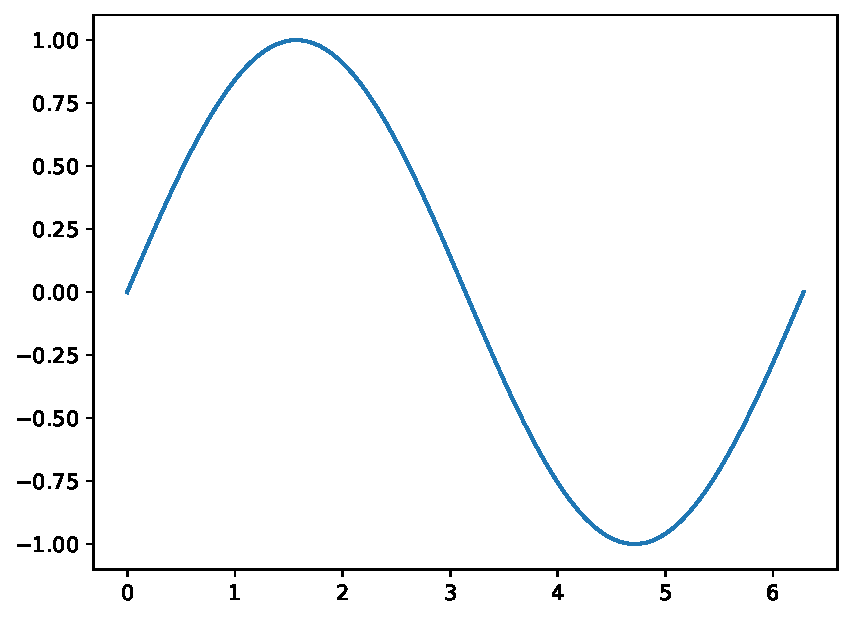
\includegraphics[width=0.7\linewidth]{fig/matplotlib0.pdf}
    \end{samepage}
\end{figure}
\end{frame}

\begin{frame}
  \frametitle{Matplotlib - Labels}
  We can add labels to the axes a legend and a title to the plot:
  \lstinputlisting[language=python, firstline=6,lastline=14]{examples/matplotlib1.py}
  Documentation: \hrefu{https://matplotlib.org/stable/api/_as_gen/matplotlib.pyplot.title.html}{\texttt{title()}}, \hrefu{https://matplotlib.org/stable/api/_as_gen/matplotlib.pyplot.xlabel.html}{\texttt{xlabel()}}, \hrefu{https://matplotlib.org/stable/api/_as_gen/matplotlib.pyplot.ylabel.html}{\texttt{ylabel()}}, \hrefu{https://matplotlib.org/stable/api/_as_gen/matplotlib.pyplot.legend.html}{\texttt{legend()}}
\end{frame}

\begin{frame}
  \frametitle{Matplotlib - Labels}
  \begin{figure}[H]
    \centering
    \begin{samepage}
        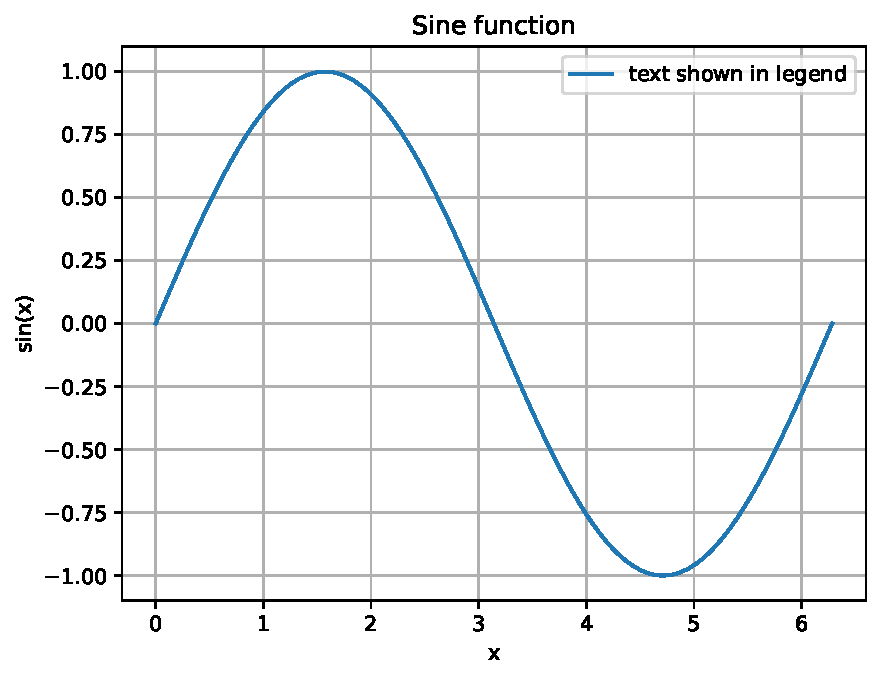
\includegraphics[width=0.7\linewidth]{fig/matplotlib1.pdf}
    \end{samepage}
\end{figure}
\end{frame}

\begin{frame}
  \frametitle{Matplotlib - Save figures}
  To save plotted figures, use the \hrefu{https://matplotlib.org/stable/api/_as_gen/matplotlib.pyplot.savefig.html}{\texttt{savefig()}} function:
  \lstinputlisting[language=python, firstline=2]{examples/matplotlib2.py}

\begin{minipage}[t]{0.35\textwidth}
    \vspace{-3.5cm}
    Or use the floppy disk symbols in the pop-up windows
\end{minipage}
\hfill
\begin{minipage}[t]{0.6\textwidth}
    \centering
    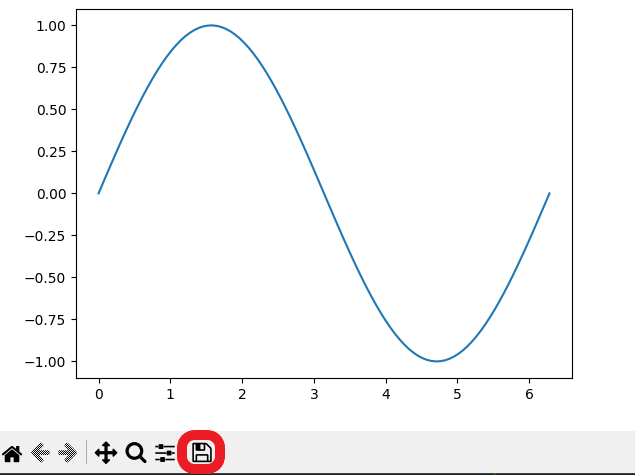
\includegraphics[width=\linewidth]{fig/Saveplot.png}
\end{minipage}
\end{frame}

\begin{frame}
  \frametitle{Matplotlib - Plotoptions}
  \hrefu{https://matplotlib.org/stable/api/_as_gen/matplotlib.pyplot.plot.html}{\texttt{plot()}} function has many options to customize the plot. Format strings \texttt{fmt = '[marker][line][color]'} change the appearance of the lines:\\
  \lstinputlisting[language=python, firstline=3, lastline=9]{examples/matplotlib3.py}
\end{frame}

\begin{frame}
  \frametitle{Matplotlib - Plotoptions}
  Using the plot options from the last slide we get:
  \begin{figure}[H]
    \centering
    \begin{samepage}
        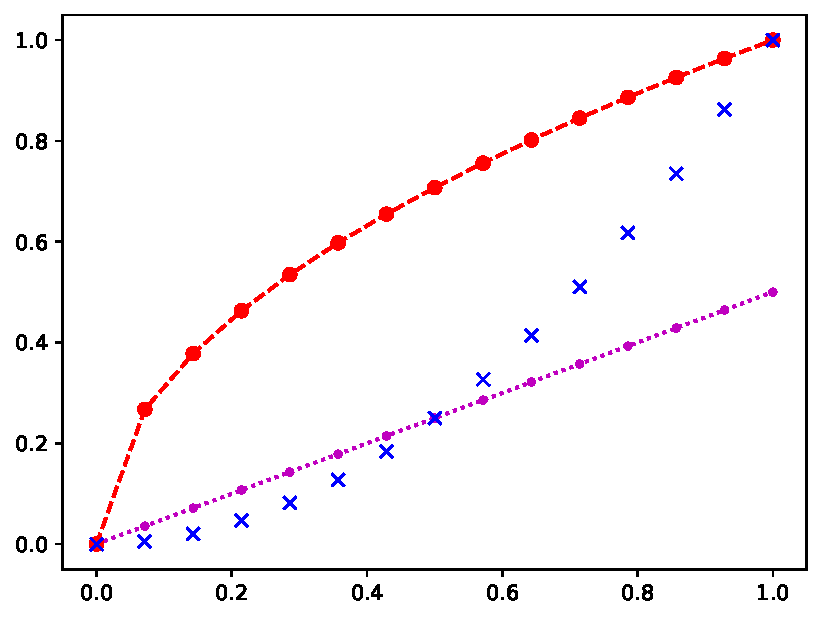
\includegraphics[width=0.65\linewidth]{fig/matplotlib3.pdf}
    \end{samepage}
\end{figure}
\end{frame}

\begin{frame}
  \frametitle{Matplotlib - Markers/Linestyles/Colors}
  Some markers: \texttt{.} (point), \texttt{o} (circle), \texttt{+} (plus), \texttt{*} (star), \texttt{s} (square), \texttt{p} (pentagon), \texttt{h} (hexagon 1), \texttt{H} (hexagon 2)\\\vspace{5mm}
  Line styles: \texttt{-} (solid line), \texttt{--} (dashed line),\\\texttt{-.} (dash-dot line), \texttt{:} (dotted line)\\\vspace{5mm}
  Colors: \texttt{b} (blue), \texttt{g} (green), \texttt{r} (red), \texttt{c} (cyan),\\\texttt{m} (magenta), \texttt{y} (yellow), \texttt{k} (black), \texttt{w} (white)\\
\end{frame}
\section{File I/O}
\begin{frame}
  \frametitle{Reading and writing files}
  %numpy loadtxt
  \hrefu{https://numpy.org/doc/stable/reference/generated/numpy.loadtxt.html}{loadtxt} can be used to read data from a text file.\\
  \lstinputlisting[language=python, firstline=2]{examples/read\_write.py}
\end{frame}
\begin{frame}
  \frametitle{Reading csv files -- input}
  \begin{figure}[H]
    \centering
    \begin{samepage}
        \includegraphics[width=0.5\linewidth]{fig/csv\_example.png}
    \end{samepage}
\end{figure}
\end{frame}
\begin{frame}
  \frametitle{Reading csv files}
  \hrefu{https://numpy.org/doc/stable/reference/generated/numpy.genfromtxt.html}{genfromtxt} can be used to read data from a csv file.\\
  \lstinputlisting[language=python, firstline=3, lastline=10]{examples/simple\_csv.py}
\end{frame}
\begin{frame}
  \frametitle{Reading csv files -- output}
  \begin{figure}[H]
    \centering
    \begin{samepage}
        \includegraphics[width=0.7\linewidth]{fig/simple\_example.pdf}
    \end{samepage}
\end{figure}
\end{frame}
\section{Numpy (extra)}
\begin{frame}
  \frametitle{Ravel vs.Flatten}
  \hrefu{https://numpy.org/doc/stable/reference/generated/numpy.ravel.html}{ravel} returns a view of the original array. \hrefu{https://numpy.org/doc/stable/reference/generated/numpy.ndarray.flatten.html}{flatten} returns a \textbf{copy} of the original array.
  \lstinputlisting[language=python, firstline=3]{examples/numpy6.py}
\end{frame}
\begin{frame}
  \frametitle{Numpy examples -- all \& any}
  \hrefu{https://numpy.org/doc/stable/reference/generated/numpy.all.html}{all} and \hrefu{https://numpy.org/doc/stable/reference/generated/numpy.any.html}{any} can be used to check if all or any elements of an array comply with a condition.
  \lstinputlisting[language=python, firstline=3]{examples/numpy3.py}
\end{frame}
%%%%%%%%%%%%%%%%%%%%%%%%%%%%%%%%%%%%%%%%%%%%%%%%%%%%%%%%%%%%%%%%%%%%%%%%%%%%
\end{document}
%%%%%%%%%%%%%%%%%%%%%%%%%%%%%%%%%%%%%%%%%%%%%%%%%%%%%%%%%%%%%%%%%%%%%%%%%%%%

%% EOF
